\section{Reproducibility Details}
\label{app:reproducibility}

All experiments used CIFAR-100 in a fixed ten-task class-incremental
partition of ten classes per task. The class partition was determined by split
seed 13 and was shared by all runs; the three reported seeds therefore vary
training randomness rather than class order. Each task was trained with a
ResNet-18 (64 base filters, no dropout), batch size 128, mixed-precision
arithmetic, and SGD with learning rate 0.1, momentum 0.9, weight decay
$5\times10^{-4}$, and gradient clipping at 1.0. No learning-rate schedule or
warm-up was used. The configured task length was 70 epochs. Run metadata
records 71 epochs for every seed because the trainer's epoch counter was
incremented once after the final configured epoch; this recording discrepancy
does not alter the configured schedule.

Unless an ablation changes the relevant component, models use the cosine-margin
head (scale 30, margin 0.35) with weight imprinting of each new task's head rows
(after task 0, which retains its random initialization), a distillation weight
of 1 at temperature 2, and a retrieval budget of 64. The no-distillation
ablation sets the distillation weight to zero; the linear-head ablation replaces
the cosine-margin head. The static-bank baseline and the head-logit evaluation
ablation use head-logit prediction; all other reported configurations use NME
prediction. Table~\ref{tab:app-protocol} gives the remaining protocol settings.

\begin{table}[t]
  \centering
  \caption{Protocol settings shared across runs unless an ablation explicitly
  changes them.}
  \label{tab:app-protocol}
  \small
  \resizebox{\linewidth}{!}{%
  \begin{tabular}{ll}
    \toprule
    Setting & Value \\
    \midrule
    Dataset and partition & CIFAR-100; 10 tasks $\times$ 10 classes; split seed 13 \\
    Probe / validation split & 30 / 20 \\
    Backbone & ResNet-18; 64 base filters; dropout 0 \\
    Optimizer & SGD; lr 0.1; momentum 0.9; weight decay $5\times10^{-4}$ \\
    Training & 70 configured epochs per task; batch size 128; gradient clip 1.0 \\
    Precision & 16-mixed \\
    Random seeds & 1993, 2023, 42 \\
    Default exemplar budget & 2,000 \\
    Default retrieval budget & 64 \\
    Hardware & Tesla T4 \\
    Software & Python 3.12.13; PyTorch 2.11.0+cu128; Lightning 2.6.5 \\
    \bottomrule
  \end{tabular}
  }
\end{table}

\section{Task-Level Results}
\label{app:task-results}

For task $i$, the reported forgetting is the difference between the best
accuracy attained on task $i$ during training and its accuracy after the final
task. Figure~\ref{fig:app-forgetting} gives this quantity for every method and
task. The final task has zero forgetting by construction. The figure therefore
separates aggregate retention from its distribution over task age and avoids
inferring a trajectory from a single summary statistic.

\begin{figure}[t]
  \centering
  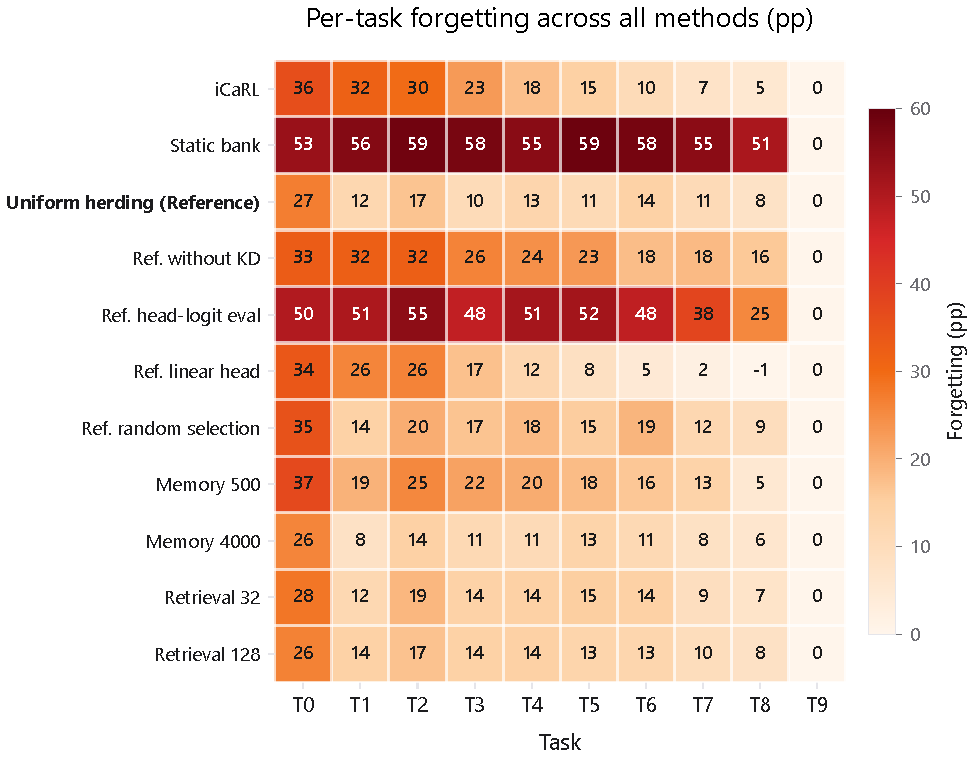
\includegraphics[width=\linewidth]{data/appendix/figures/figA1_forgetting_heatmap.pdf}
  \caption{Per-task forgetting, in percentage points, for all evaluated
  configurations. Each entry is the drop from the task's best observed accuracy
  to its final accuracy. Task T9 is zero by definition because it is introduced
  last.}
  \label{fig:app-forgetting}
\end{figure}

Figures~\ref{fig:app-reference-evolution} and~\ref{fig:app-icarl-evolution}
show the complete task-by-time accuracy matrices for the reference method and
iCaRL, respectively. Row $i$, column $t$ is the accuracy on task $i$ after
learning through task $t$; cells with $i>t$ are undefined and omitted. These
matrices are the underlying trajectories from which the task-level forgetting
values are calculated.

\begin{figure}[t]
  \centering
  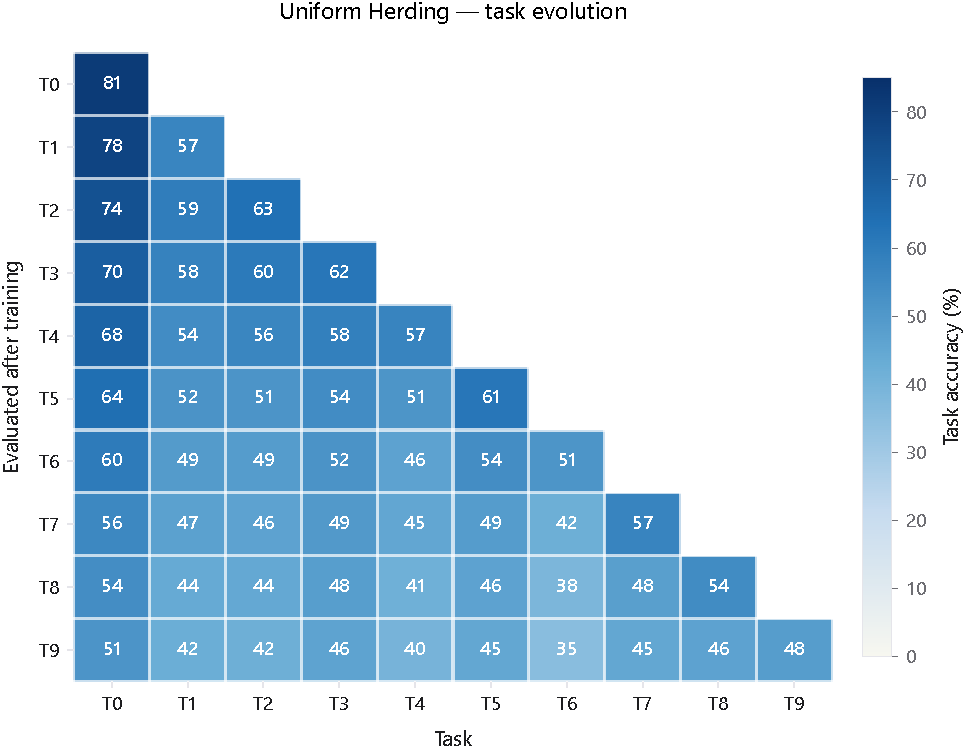
\includegraphics[width=\linewidth]{data/appendix/figures/figA2_evolution_reference.pdf}
  \caption{Task-evolution accuracy matrix for uniform herding with NME
  prediction (the reference configuration).}
  \label{fig:app-reference-evolution}
\end{figure}

\begin{figure}[t]
  \centering
  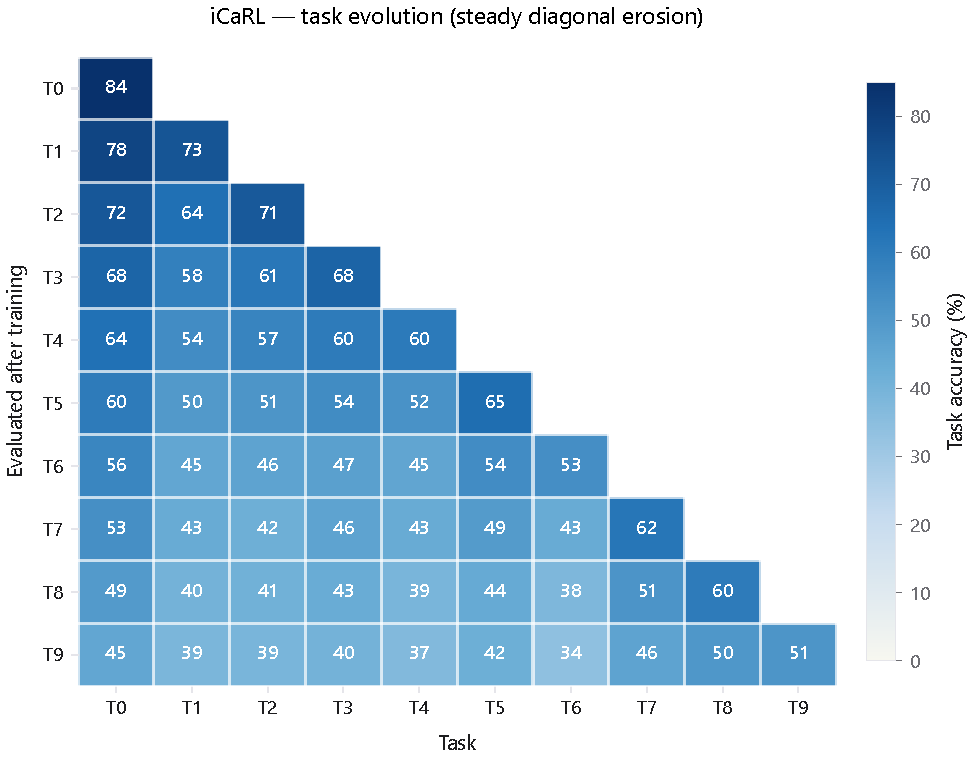
\includegraphics[width=\linewidth]{data/appendix/figures/figA3_evolution_icarl.pdf}
  \caption{Task-evolution accuracy matrix for iCaRL.}
  \label{fig:app-icarl-evolution}
\end{figure}

Figure~\ref{fig:app-kd-slopes} provides a seed-level view of the principal
stability comparison. For each earlier task and each seed, it connects the
accuracy at introduction with the final accuracy. It is a visualization of the
same per-seed measurements summarized in the main text, not an additional
statistical test.

\begin{figure}[t]
  \centering
  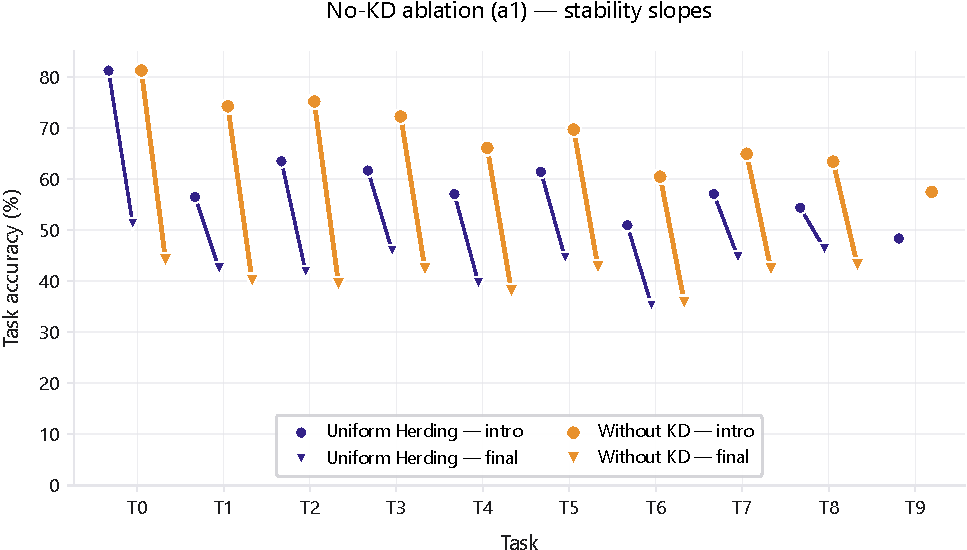
\includegraphics[width=\linewidth]{data/appendix/figures/figA4_stability_slopes.pdf}
  \caption{Seed-level task trajectories for the reference configuration and the
  no-distillation ablation. Lines connect task-introduction accuracy to final
  accuracy for the same task and seed.}
  \label{fig:app-kd-slopes}
\end{figure}

\section{Seed-Level Outcomes and Compute}
\label{app:seed-compute}

Table~\ref{tab:app-seeds} reports the raw aggregate metrics for every run and
seed. Values are percentages. This table is included to make the means and
standard deviations in the main text auditable without treating the three
training seeds as independent task-level observations.

\begin{table}[t]
  \centering
  \caption{Per-seed final average accuracy, forgetting, and backward transfer.}
  \label{tab:app-seeds}
  \scriptsize
  \begin{tabular}{llrrr}
    \toprule
    ID & Configuration / seed & Average accuracy & Forgetting & BWT \\
    \midrule
    B1 & iCaRL / 1993 & 42.29 & 19.50 & -19.50 \\
    B1 & iCaRL / 2023 & 43.46 & 19.32 & -19.32 \\
    B1 & iCaRL / 42 & 41.33 & 19.56 & -19.56 \\
    B2 & Static bank / 1993 & 28.15 & 56.34 & -56.34 \\
    B2 & Static bank / 2023 & 30.43 & 53.93 & -53.93 \\
    B2 & Static bank / 42 & 27.22 & 57.31 & -57.31 \\
    B3 & Reference / 1993 & 45.11 & 13.37 & -13.17 \\
    B3 & Reference / 2023 & 46.16 & 13.77 & -13.38 \\
    B3 & Reference / 42 & 43.71 & 14.42 & -14.09 \\
    a1 & No KD / 1993 & 45.22 & 23.68 & -23.68 \\
    a1 & No KD / 2023 & 44.54 & 25.07 & -25.07 \\
    a1 & No KD / 42 & 44.60 & 25.59 & -25.59 \\
    a2 & Head-logit / 1993 & 33.09 & 48.07 & -48.07 \\
    a2 & Head-logit / 2023 & 34.93 & 46.83 & -46.83 \\
    a2 & Head-logit / 42 & 35.81 & 44.17 & -44.17 \\
    a3 & Linear head / 1993 & 43.77 & 15.07 & -14.70 \\
    a3 & Linear head / 2023 & 44.02 & 14.97 & -14.82 \\
    a3 & Linear head / 42 & 42.92 & 14.00 & -13.50 \\
    a4 & Random selection / 1993 & 39.94 & 18.31 & -17.90 \\
    a4 & Random selection / 2023 & 40.35 & 19.11 & -18.20 \\
    a4 & Random selection / 42 & 40.21 & 17.62 & -17.16 \\
    s1 & Memory 500 / 1993 & 36.64 & 18.24 & -18.24 \\
    s1 & Memory 500 / 2023 & 37.33 & 20.61 & -20.61 \\
    s1 & Memory 500 / 42 & 36.51 & 20.02 & -20.02 \\
    s2 & Memory 4000 / 1993 & 47.60 & 11.40 & -10.93 \\
    s2 & Memory 4000 / 2023 & 48.56 & 12.68 & -12.33 \\
    s2 & Memory 4000 / 42 & 46.81 & 13.93 & -13.10 \\
    s3 & Retrieval 32 / 1993 & 43.46 & 13.99 & -13.92 \\
    s3 & Retrieval 32 / 2023 & 43.92 & 16.33 & -15.86 \\
    s3 & Retrieval 32 / 42 & 42.46 & 14.62 & -14.24 \\
    s4 & Retrieval 128 / 1993 & 44.57 & 13.62 & -13.52 \\
    s4 & Retrieval 128 / 2023 & 45.86 & 15.03 & -14.66 \\
    s4 & Retrieval 128 / 42 & 44.00 & 15.33 & -14.96 \\
    \bottomrule
  \end{tabular}
\end{table}

Table~\ref{tab:app-compute} reports elapsed wall-clock time per run on a Tesla
T4. These timings describe the implementation and hardware used here; they are
not intended as hardware-independent efficiency comparisons.

\begin{table}[t]
  \centering
  \caption{Wall-clock time per run in seconds (mean $\pm$ standard deviation
  across the three seeds), measured on a Tesla T4.}
  \label{tab:app-compute}
  \small
  \begin{tabular}{llr}
    \toprule
    ID & Configuration & Seconds \\
    \midrule
    B1 & iCaRL & $3754.8 \pm 38.0$ \\
    B2 & Static bank & $2716.3 \pm 91.6$ \\
    B3 & Reference & $4493.2 \pm 52.5$ \\
    a1 & No KD & $3307.7 \pm 54.0$ \\
    a2 & Head-logit & $4279.5 \pm 93.4$ \\
    a3 & Linear head & $3732.1 \pm 42.7$ \\
    a4 & Random selection & $4555.9 \pm 37.1$ \\
    s1 & Memory 500 & $4292.4 \pm 54.2$ \\
    s2 & Memory 4000 & $4351.7 \pm 26.0$ \\
    s3 & Retrieval 32 & $3958.1 \pm 104.2$ \\
    s4 & Retrieval 128 & $5919.2 \pm 49.9$ \\
    \bottomrule
  \end{tabular}
\end{table}

\section{Exemplar Quotas}
\label{app:quotas}

After task $t$, the available memory is divided among the $10(t+1)$ observed
classes. Table~\ref{tab:app-quotas} lists the resulting per-class quotas. When
the budget is not divisible by the number of observed classes, the allocation
uses floor rounding and adjacent classes can differ by one exemplar.

\begin{table}[t]
  \centering
  \caption{Per-class exemplar quota after each task. Ranges indicate the
  one-exemplar difference induced by floor rounding.}
  \label{tab:app-quotas}
  \small
  \resizebox{\linewidth}{!}{%
  \begin{tabular}{lrrrrrrrrrr}
    \toprule
    Budget & T0 & T1 & T2 & T3 & T4 & T5 & T6 & T7 & T8 & T9 \\
    \midrule
    500 & 50 & 25 & 16--17 & 12--13 & 10 & 8--9 & 7--8 & 6--7 & 5--6 & 5 \\
    2,000 & 200 & 100 & 66--67 & 50 & 40 & 33--34 & 28--29 & 25 & 22--23 & 20 \\
    4,000 & 400 & 200 & 133--134 & 100 & 80 & 66--67 & 57--58 & 50 & 44--45 & 40 \\
    \bottomrule
  \end{tabular}
  }
\end{table}
